\documentclass[14pt]{extbook}
\usepackage{multicol, enumerate, enumitem, hyperref, color, soul, setspace, parskip, fancyhdr} %General Packages
\usepackage{amssymb, amsthm, amsmath, bbm, latexsym, units, mathtools} %Math Packages
\everymath{\displaystyle} %All math in Display Style
% Packages with additional options
\usepackage[headsep=0.5cm,headheight=12pt, left=1 in,right= 1 in,top= 1 in,bottom= 1 in]{geometry}
\usepackage[usenames,dvipsnames]{xcolor}
\usepackage{dashrule}  % Package to use the command below to create lines between items
\newcommand{\litem}[1]{\item#1\hspace*{-1cm}\rule{\textwidth}{0.4pt}}
\pagestyle{fancy}
\lhead{Progress Quiz 4}
\chead{}
\rhead{Version B}
\lfoot{8448-1521}
\cfoot{}
\rfoot{Fall 2020}
\begin{document}

\begin{enumerate}
\litem{
Graph the equation below.\[ f(x) = -(x+4)^2 - 19 \]\begin{enumerate}[label=\Alph*.]
\begin{multicols}{2}\item 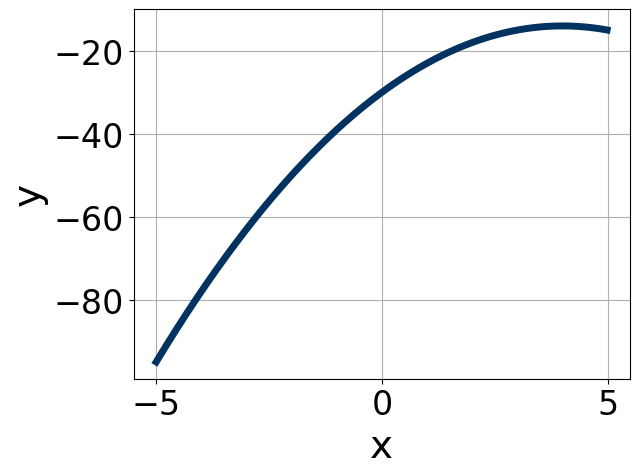
\includegraphics[width = 0.3\textwidth]{../Figures/quadraticEquationToGraphCopyAB.png}\item 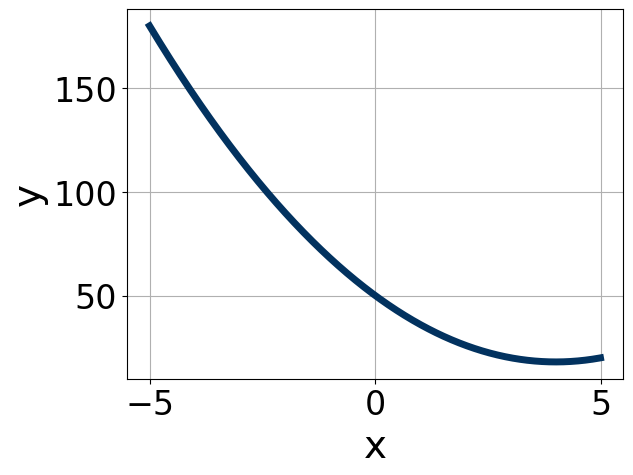
\includegraphics[width = 0.3\textwidth]{../Figures/quadraticEquationToGraphCopyBB.png}\item 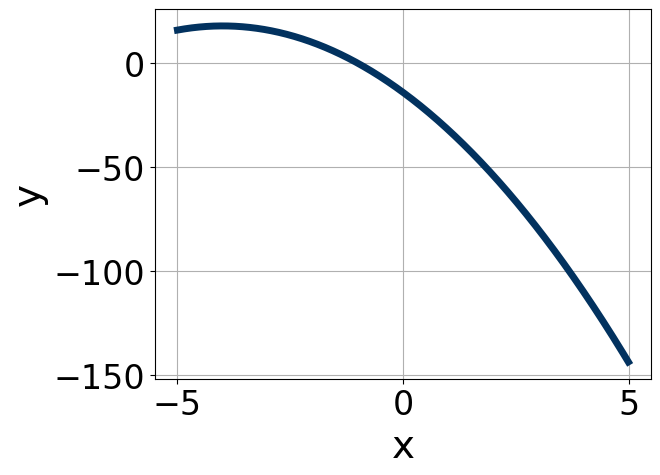
\includegraphics[width = 0.3\textwidth]{../Figures/quadraticEquationToGraphCopyCB.png}\item 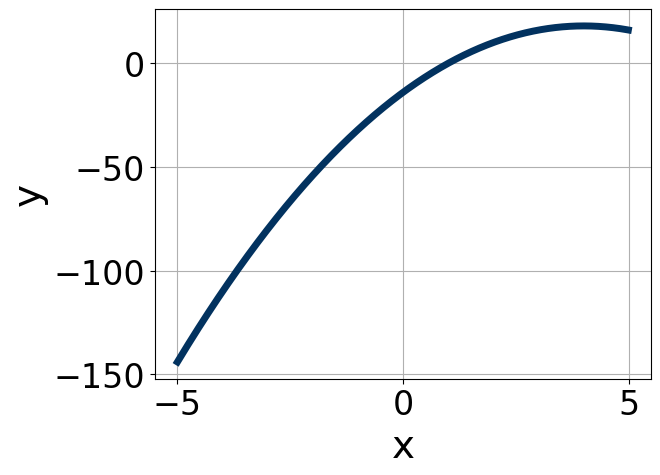
\includegraphics[width = 0.3\textwidth]{../Figures/quadraticEquationToGraphCopyDB.png}\end{multicols}\item None of the above.
\end{enumerate} }
\litem{
Write the equation of the graph presented below in the form $f(x)=ax^2+bx+c$, assuming  $a=1$ or $a=-1$. Then, choose the intervals that $a, b,$ and $c$ belong to.
\begin{center}
    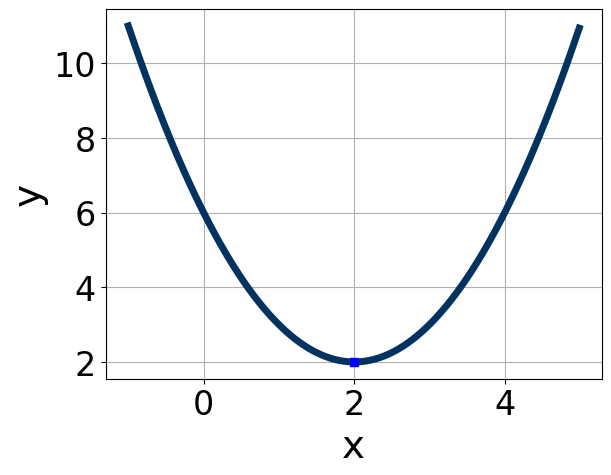
\includegraphics[width=0.5\textwidth]{../Figures/quadraticGraphToEquationCopyB.png}
\end{center}
\begin{enumerate}[label=\Alph*.]
\item \( a \in [-1.7, -0.8], \hspace*{5mm} b \in [3, 6], \text{ and } \hspace*{5mm} c \in [0, 5] \)
\item \( a \in [0.9, 1.5], \hspace*{5mm} b \in [-6, -3], \text{ and } \hspace*{5mm} c \in [0, 5] \)
\item \( a \in [-1.7, -0.8], \hspace*{5mm} b \in [-6, -3], \text{ and } \hspace*{5mm} c \in [-8, -3] \)
\item \( a \in [0.9, 1.5], \hspace*{5mm} b \in [3, 6], \text{ and } \hspace*{5mm} c \in [0, 5] \)
\item \( a \in [-1.7, -0.8], \hspace*{5mm} b \in [3, 6], \text{ and } \hspace*{5mm} c \in [-8, -3] \)

\end{enumerate} }
\litem{
Solve the quadratic equation below. Then, choose the intervals that the solutions belong to, with $x_1 \leq x_2$ (if they exist).\[ 15x^{2} -9 x -5 = 0 \]\begin{enumerate}[label=\Alph*.]
\item \( x_1 \in [-0.72, -0.3] \text{ and } x_2 \in [0.7, 1.8] \)
\item \( x_1 \in [-1.29, -0.91] \text{ and } x_2 \in [0.3, 0.4] \)
\item \( x_1 \in [-19.36, -18.47] \text{ and } x_2 \in [19.2, 21.7] \)
\item \( x_1 \in [-5.71, -5.07] \text{ and } x_2 \in [13.4, 14.5] \)
\item \( \text{There are no Real solutions.} \)

\end{enumerate} }
\litem{
Solve the quadratic equation below. Then, choose the intervals that the solutions belong to, with $x_1 \leq x_2$ (if they exist).\[ -15x^{2} -15 x + 2 = 0 \]\begin{enumerate}[label=\Alph*.]
\item \( x_1 \in [-0.28, 0.82] \text{ and } x_2 \in [0.27, 1.5] \)
\item \( x_1 \in [-2.09, -1.73] \text{ and } x_2 \in [16.04, 16.8] \)
\item \( x_1 \in [-19.34, -18.54] \text{ and } x_2 \in [17.52, 19.11] \)
\item \( x_1 \in [-1.53, -0.47] \text{ and } x_2 \in [-0.45, 1.06] \)
\item \( \text{There are no Real solutions.} \)

\end{enumerate} }
\litem{
Factor the quadratic below. Then, choose the intervals that contain the constants in the form $(ax+b)(cx+d); b \leq d.$\[ 24x^{2} +50 x + 25 \]\begin{enumerate}[label=\Alph*.]
\item \( a \in [5.77, 6.9], \hspace*{5mm} b \in [2, 14], \hspace*{5mm} c \in [3.6, 4.15], \text{ and } \hspace*{5mm} d \in [1, 7] \)
\item \( a \in [11.52, 13.7], \hspace*{5mm} b \in [2, 14], \hspace*{5mm} c \in [1.41, 2.41], \text{ and } \hspace*{5mm} d \in [1, 7] \)
\item \( a \in [-0.7, 1.21], \hspace*{5mm} b \in [18, 26], \hspace*{5mm} c \in [0.67, 1.76], \text{ and } \hspace*{5mm} d \in [30, 34] \)
\item \( a \in [1.39, 2.59], \hspace*{5mm} b \in [2, 14], \hspace*{5mm} c \in [10.77, 12.36], \text{ and } \hspace*{5mm} d \in [1, 7] \)
\item \( \text{None of the above.} \)

\end{enumerate} }
\litem{
Solve the quadratic equation below. Then, choose the intervals that the solutions $x_1$ and $x_2$ belong to, with $x_1 \leq x_2$.\[ 15x^{2} +38 x + 24 = 0 \]\begin{enumerate}[label=\Alph*.]
\item \( x_1 \in [-2.61, -2.3] \text{ and } x_2 \in [-0.78, -0.62] \)
\item \( x_1 \in [-20.02, -19.93] \text{ and } x_2 \in [-18.12, -17.96] \)
\item \( x_1 \in [-6.26, -5.92] \text{ and } x_2 \in [-0.29, -0.25] \)
\item \( x_1 \in [-1.57, -1.24] \text{ and } x_2 \in [-1.22, -1.16] \)
\item \( x_1 \in [-2.79, -2.45] \text{ and } x_2 \in [-0.65, -0.55] \)

\end{enumerate} }
\litem{
Factor the quadratic below. Then, choose the intervals that contain the constants in the form $(ax+b)(cx+d); b \leq d.$\[ 36x^{2} -65 x + 25 \]\begin{enumerate}[label=\Alph*.]
\item \( a \in [0.65, 1.07], \hspace*{5mm} b \in [-50, -43], \hspace*{5mm} c \in [0.04, 1.62], \text{ and } \hspace*{5mm} d \in [-24, -18] \)
\item \( a \in [1.49, 3.1], \hspace*{5mm} b \in [-8, -4], \hspace*{5mm} c \in [11.15, 12.41], \text{ and } \hspace*{5mm} d \in [-7, 4] \)
\item \( a \in [8.23, 9.74], \hspace*{5mm} b \in [-8, -4], \hspace*{5mm} c \in [2.63, 4.9], \text{ and } \hspace*{5mm} d \in [-7, 4] \)
\item \( a \in [17.09, 19.35], \hspace*{5mm} b \in [-8, -4], \hspace*{5mm} c \in [1.61, 3.66], \text{ and } \hspace*{5mm} d \in [-7, 4] \)
\item \( \text{None of the above.} \)

\end{enumerate} }
\litem{
Graph the equation below.\[ f(x) = (x+1)^2 - 11 \]\begin{enumerate}[label=\Alph*.]
\begin{multicols}{2}\item 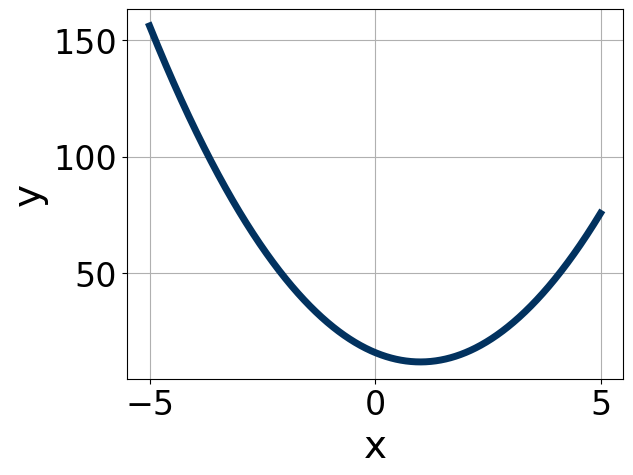
\includegraphics[width = 0.3\textwidth]{../Figures/quadraticEquationToGraphAB.png}\item 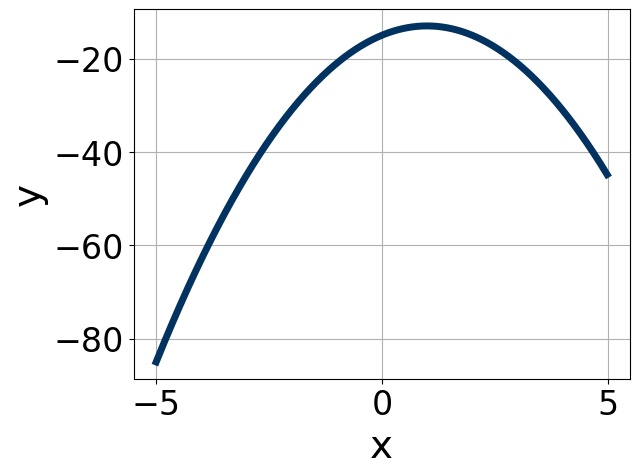
\includegraphics[width = 0.3\textwidth]{../Figures/quadraticEquationToGraphBB.png}\item 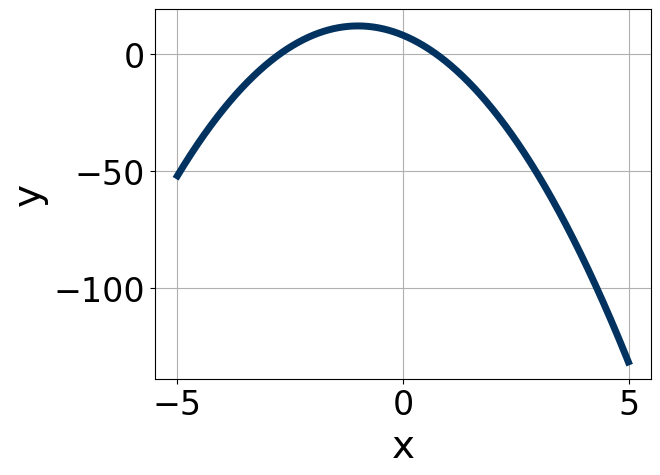
\includegraphics[width = 0.3\textwidth]{../Figures/quadraticEquationToGraphCB.png}\item 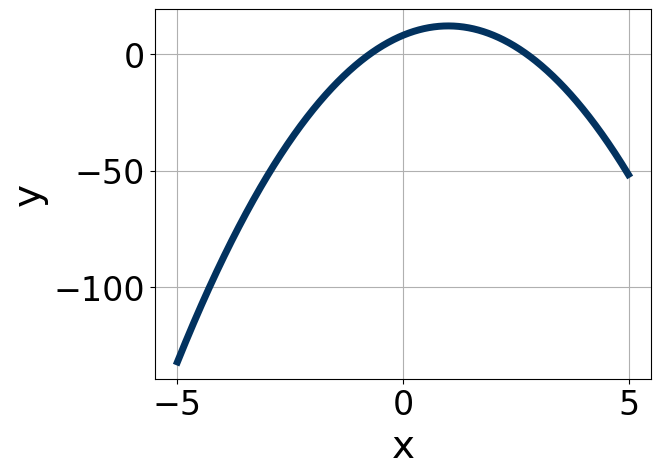
\includegraphics[width = 0.3\textwidth]{../Figures/quadraticEquationToGraphDB.png}\end{multicols}\item None of the above.
\end{enumerate} }
\litem{
Write the equation of the graph presented below in the form $f(x)=ax^2+bx+c$, assuming  $a=1$ or $a=-1$. Then, choose the intervals that $a, b,$ and $c$ belong to.
\begin{center}
    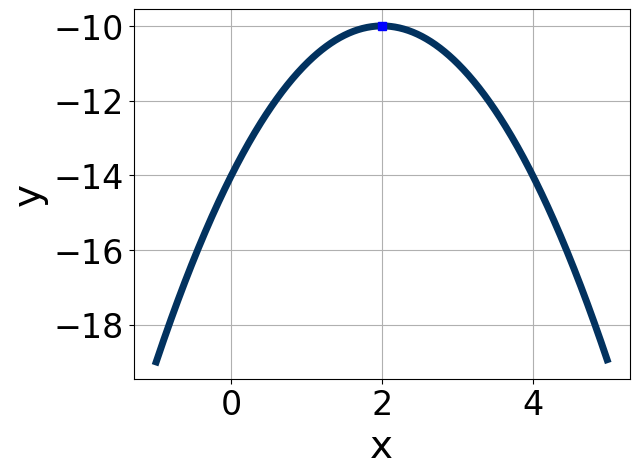
\includegraphics[width=0.5\textwidth]{../Figures/quadraticGraphToEquationB.png}
\end{center}
\begin{enumerate}[label=\Alph*.]
\item \( a \in [-4, 0], \hspace*{5mm} b \in [-9, -7], \text{ and } \hspace*{5mm} c \in [-19, -14] \)
\item \( a \in [-4, 0], \hspace*{5mm} b \in [7, 10], \text{ and } \hspace*{5mm} c \in [-19, -14] \)
\item \( a \in [0, 5], \hspace*{5mm} b \in [7, 10], \text{ and } \hspace*{5mm} c \in [13, 15] \)
\item \( a \in [0, 5], \hspace*{5mm} b \in [7, 10], \text{ and } \hspace*{5mm} c \in [18, 21] \)
\item \( a \in [0, 5], \hspace*{5mm} b \in [-9, -7], \text{ and } \hspace*{5mm} c \in [13, 15] \)

\end{enumerate} }
\litem{
Solve the quadratic equation below. Then, choose the intervals that the solutions $x_1$ and $x_2$ belong to, with $x_1 \leq x_2$.\[ 10x^{2} -57 x + 54 = 0 \]\begin{enumerate}[label=\Alph*.]
\item \( x_1 \in [11.91, 12.15] \text{ and } x_2 \in [43.44, 45.42] \)
\item \( x_1 \in [-0.16, 0.5] \text{ and } x_2 \in [12.69, 13.52] \)
\item \( x_1 \in [0.72, 1.03] \text{ and } x_2 \in [5.54, 7.31] \)
\item \( x_1 \in [1.29, 1.61] \text{ and } x_2 \in [1.9, 3.63] \)
\item \( x_1 \in [1.04, 1.26] \text{ and } x_2 \in [3.78, 5.27] \)

\end{enumerate} }
\end{enumerate}

\end{document}